\section{Dwelling (envelope) model analogous to a 2R-2C network}

The 2R-2C house model structure is implemented as described below:
	
\begin{figure}[H]
	\centering
	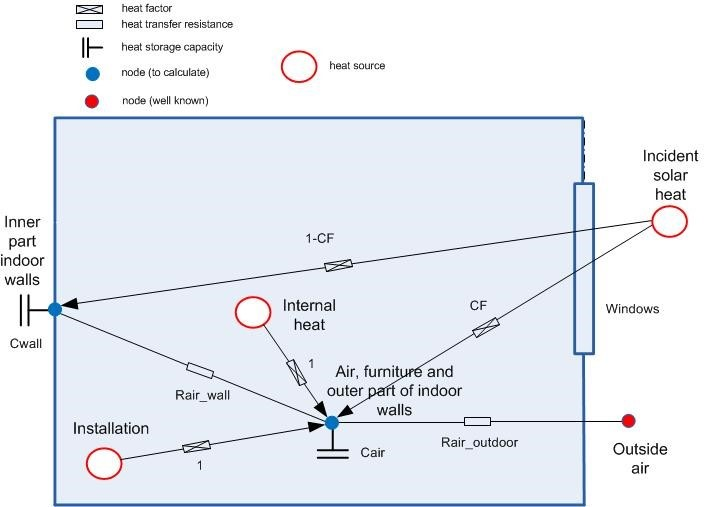
\includegraphics[width=1.0\columnwidth]{Pictures/envelopRC.jpg}
	\caption[Short title]{Schematic of envelope model}
	\label{fig:envelope2R2C}
	\end{figure} 
	
The equivalent electrical 2R-2C network with components and topology is given in Fig. \ref{fig:elec2R2C}.

\begin{figure}[H]
	\centering
	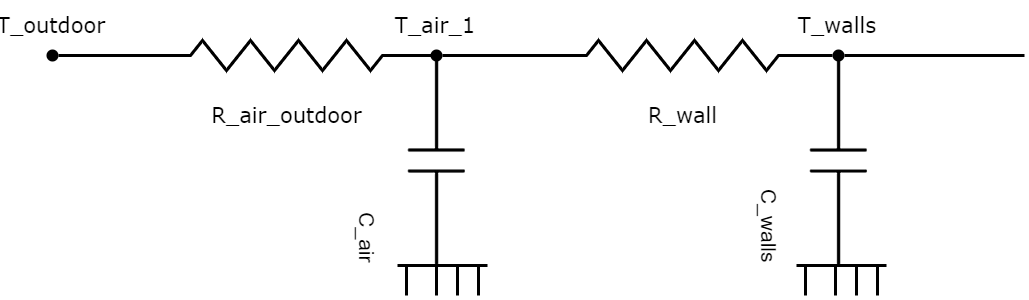
\includegraphics[width=1.0\columnwidth]{Pictures/2R2C_Model.png}
	\caption[Short title]{2R-2C house model}
	\label{fig:elec2R2C}
	\end{figure}
	
The model consists of two capacitances C\textsubscript{air, indoor} and C\textsubscript{wall} and two resistances R\textsubscript{wall} and R\textsubscript{air, outdoor}. The incident solar energy is divided between C\textsubscript{wall} and C\textsubscript{air} through the convection factor CF. It is assumed that both internal heat (lighting, occupancy and electric devices) and supplied heat (installation) initially heat up the indoor air. In Fig. \ref{fig:elec2R2C}, they are fully released at the T\textsubscript{air} node. 

 It is also assumed that furniture and the surface part of the walls have the same temperature as the air and the wall mass is divided between the air and wall mass. Thus, the capacity of the air node consists of the air capacity, furniture capacity and capacity of a part of the walls. \textbf{Appendix A} presents the coefficients in the dwelling model. In the resistance R\textsubscript{air, outdoor} the influence of heat transmission through the outdoor walls and natural ventilation is considered. 
 
For the air and wall nodes the following energy balances can be set up: 

\begin{equation}
C_{air}\frac{dT_{air}}{dt}=\frac{T_{outdoor}-T_{air}}{R_{air_{\_}outdoor}} + \frac{T_{wall}-T_{air}}{R_{air_{\_}wall}} + \dot{Q}_{inst} + \dot{Q}_{internal} + CF\cdot\dot{Q}_{solar}
\end{equation}

\begin{equation}
C_{wall}\frac{dT_{wall}}{dt}=\frac{T_{air}-T_{wall}}{R_{air_{\_}wall}} + (1-CF)\cdot\dot{Q}_{solar}
\end{equation}

 \begin{itemize}
      \item CF: Convection factor (solar radiation): the convection factor is the part of the solar radiation that enters the room and is released directly convectively into the room
      \item $\dot{Q}_{inst}$: delivered heat from heating system (radiator) [W].
      \item $\dot{Q}_{solar}$: heat from solar irradiation [W].
      \item $T_{air}$: indoor air temperature $^o$C.
      \item $T_{outdoor}$: outdoor temperature $^o$C.
      \item $T_{wall}$: wall temperature $^o$C.
      \item $R_{air_{\_}wall}$: walls surface resistance [$\frac{K}{W}$].
      \item $R_{air_{\_}outdoor}$: outdoor surface resistance [$\frac{K}{W}$].
      \item $C_{air}$: air capacity [$\frac{J}{K}$].
      \item $C_{wall}$: wall capacity [$\frac{J}{K}$].
    \end{itemize}
    

Total heat transfer of solar irradiation through the glass windows. 
\begin{equation}
Q_{solar}=g.\sum(A_{glass}.q_{solar})
\end{equation}

\begin{itemize}
    \item $q_{solar}$: solar radiation on the outdoor walls [$\frac{W}{m^2}$]. 
    \item g: g value of the glass (ZTA in dutch) [0..1]\cite{zontoetreding}
    \item A: glass surface [$m^2$].
\end{itemize}

%7.6.6.1.2 Ramen met niet-verstrooiende beglazing NTA8800
%https://help.dgmr.nl/bink9/zontoetredingsfactor-zta.html
%https://www.joostdevree.nl/shtmls/zta.shtml
%ISSO-Handboek Zonnestraling: 5.5.1 en 5.2

\newpage